
\section{Approach}\label{sec-approach}

\commentws{ As previously mentioned, one major
short-coming of the state-of-the-art approaches in
detecting API compatibility issues is their inability
to analyze application-under-analysis and the
underlying ADF code in unison. As shown in
Figure~\ref{fig:compare}a, these approaches perform
analysis in two steps: analyzing the app and modeling
the ADFs.  They then perform another layer of analysis
that consider both results to detect API compatibility
issues. In doing so, these approaches can miss
detecting issues that lie deeper into the ADFs.   


\@approach, on the other hand, can analyze the
application and ADF code in unison by utilizing a novel
class-loader-based program analysis approach. A
class-loader is a runtime component that is part of any
Java or Android Virtual Machine. It is responsible for
incrementally loading any class needed during
execution. It can accomplish this because of Java
partition code into classes that can be individually
loaded. \textit{\@approach adapts this runtime
concept to support its scalable static analysis.} 

\begin{figure}[t!]
    \centering
    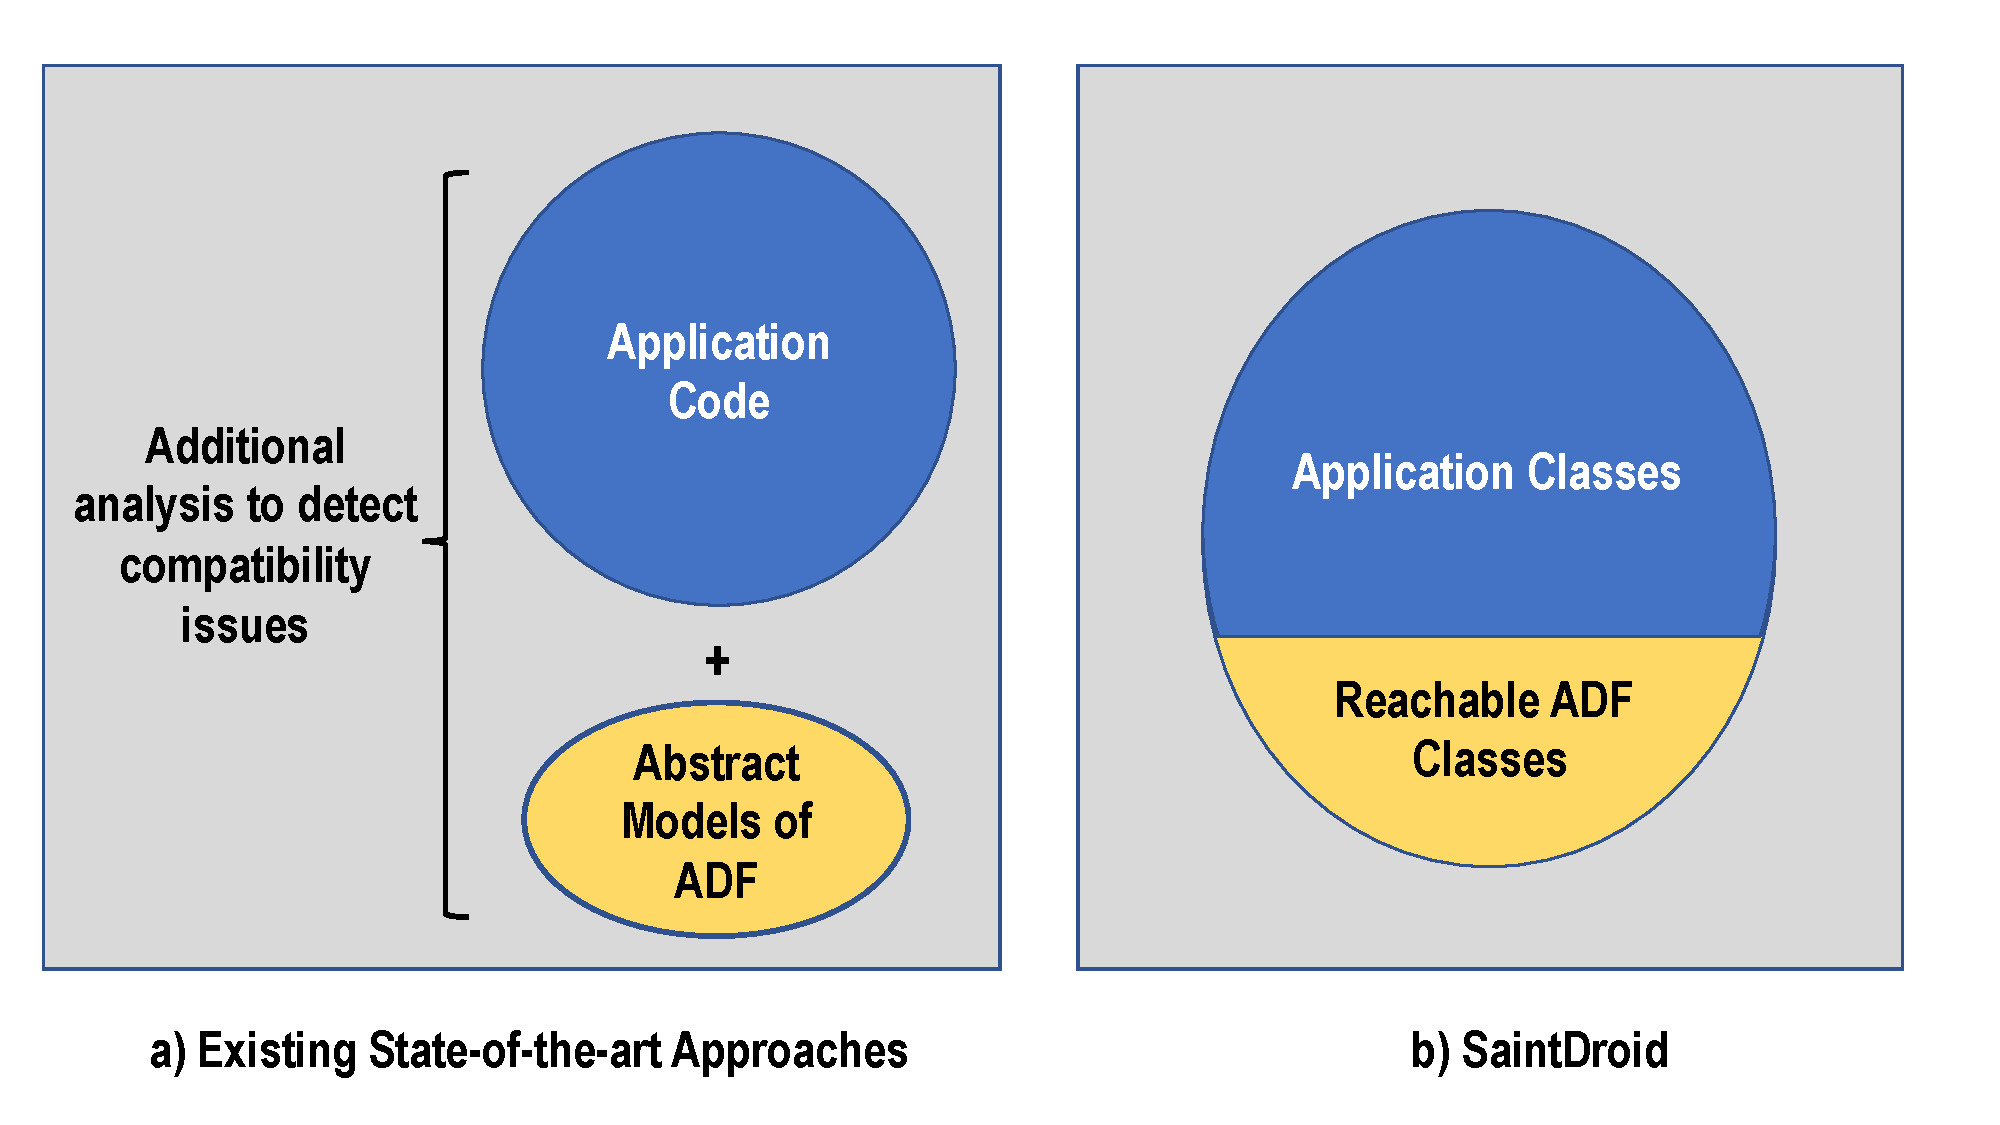
\includegraphics[width=\linewidth]{images/differences.pdf}
    \vspace{-0.2cm}
    \caption{Comparing Existing Approaches with \@approach}
    \label{fig:compare}
    \vspace{-0.3cm}
\end{figure}

In a nutshell, \@approach utilizes a \emph{ClassLoader
Virtual Machine} (\emph{CLVM}) to perform class-based
reachability analysis~\cite{tsutano2017efficient}.
\emph{CLVM} takes advantage of code structure in Java
to locate and load classes that can be reachable within
a program.  As an example, if an application method
calls an Android API, the class to which the API
belongs would be loaded.  By utilizing CLVM, \@approach
, as shown in Figure~\ref{fig:compare}b, analyzes the application classes and only the reachable
ADF classes, and not the entire ADF code. This analysis
approach significantly reduces both peak memory
footprint and memory consumption over time (as will be
shown later).  Currently, \@approach can only analyze
Dex code; it does not support the loading and analysis
of native code.  

The rest of this section overviews our approach,
leveraging CLVM to automatically detect all three types
of API- and permission-induced mismatches described in
Table~\ref{tab:api-mismatch}. As depicted in
Figure~\ref{fig:arch}, \@approach takes as input an app
APK\footnote{APK is an app bytecode package used to
distribute and install an Android application.} along
with a set of Android framework versions, and produces
a list of mismatches for the given Android app.  
\@approach comprises three main components:
}

(1) The \textit{API usage modeler (AUM)} that utilizes
different static analysis techniques, i.e., control
flow and data flow analyses, to  identify the API call
sites and the concomitant conditions thereof; 

(2) The \textit{Android revision modeler (ARM)} that
extracts essential information about the framework
APIs' lifetime and mappings between Android API calls
and the permissions required to perform those calls
from the Android framework revision history;

(3) The \textit{Android mismatch detector (AMD)} that
leverages the artifacts produced by AUM and ARM
components to effectively detect API- and
permission-related mismatches in the app under
analysis.

Next, we describe the details of each component in
turn.
 

\begin{figure}[t!]
    \centering
%    \vspace{0.2cm}
    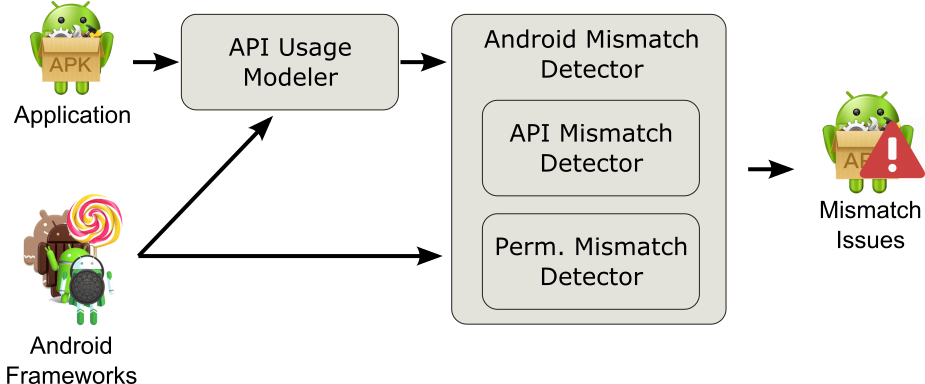
\includegraphics[width=\linewidth]{images/Approach.png}
    \vspace{-0.2cm}    
    \caption{Architecture of \@approach}
    \label{fig:arch}
    \vspace{-0.3cm}
\end{figure}

\subsection{AUM: API Usage Modeler}
\label{API Usage Extraction}

The AUM module performs path sensitive, inter-procedural
data flow analysis on call and data flow graphs of a given
decompiled APK file to determine references to API methods
or callbacks.  More precisely, AUM derives an
inter-procedural control-flow graph, augmented to account
for implicit invocations (e.g., callbacks). The produced inter-procedural
control-flow graph is further annotated with permissions
required to enact Android API calls. Finally, a reachability
analysis is conducted over the augmented graph to identify
the guards that encompass the execution paths reaching the
annotated API calls or permission-required functionalities. 

\commentty{Need more details on the analysis algorithm.
We also need to clarify the technical challenges and
our unique contributions.} 

\commentws{I add a few paragraphs to explain how our
analysis works differently than the exising state of
the art in background (at the end) and approach (at the
beginning). Please check to see if you think they
answer all the reviewer's comments from the past.}

\@approach's compatibility analysis has three major
advantages over the state-of-the-art approaches.
First,  to render our analysis more \emph{effective,
efficient, and scalable}, \@approach's AUM module
employs an approach that incrementally discovers
pertinent classes via reachability
analysis~\cite{tsutano2017efficient}.  It then analyzes
only these classes. This, in turn, allows our technique
to be significantly faster and more space efficient
than the state-of-the-art in compatibility analysis,
without sacrificing its capability in detecting
compatibility issues, as evidenced by the experimental
results (cf.  Section~\ref{sec-eval}).  Some existing
state-of-the-art
techniques~\cite{huang2018understanding,he2018understanding},
on the other hand, directly load the entire code base
into memory, and thereby facing difficulties in
handling large scale libraries such as ADF. 

%---\@approach's AUM module incrementally loads and analyzes
%classes 

Second, the AUM module analyzes actual ADF code to detect
\emph{more instances and types of compatibility issues}.
Prior work, on the other hand, focuses on creating models of
the ADF to only identify API callback compatibility
issues~\cite{huang2018understanding}.  Third, while prior
work by and large focuses on the first level framework API
calls, i.e., the first call to the framework from an
app~\cite{lili2018cid}, the AUM module analyzes method calls
beyond that initial level, which, once again, empowers
\@approach to detect \emph{more instances and types of
incompatibility issues}. 

Another key feature in Android that can affect the accuracy
of the compatibility analysis is late binding.  Indeed, apps
may dynamically load code that is not included in the main
dex file\footnote{A dex file is an executable file that
incorporates compiled code written for Android.} of the
original application package, initially loaded at the
installation time.  This mechanism enables an app to be
extended with new desirable features at run-time. However,
in spite of its virtue, it poses challenges to analysis
techniques for assessing compatibility of Android apps.

To avoid missing any potential compatibility-related issues
that may result in crashes at run-time, \@approach takes a
conservative approach and considers all possible bindings
that can be statically discovered.  More precisely,
\@approach's AUM component examines not only the main app
code loaded at the installation time, but also any other
code accessible from the app package that can be dynamically
loaded at run-time.  AUM incrementally augments the
control-flow and data-flow graphs by recursively identifying
and examining such to-be dynamically loaded classes to
ensure that every method in every such classes is analyzed.
Note that such to-be dynamically loaded code may not always
be statically analyzable, especially when it is not bundled
within installed packages, and rather externally loaded from
remote servers.
  
\subsection{ARM: Android Revision Modeler} 

The ARM module derives both the API lifecycle and the permission mapping models through mining of the Android framework revision history.
It first constructs an API database containing all public APIs defined in Android API levels 2 through 28\footnote{The Android frameworks range from API level 2 through API level 28, collected using {\it sdkmanager}, shipped with the Android SDK Tools to manage packages for the Android SDK~\cite{sdkmanager}. }, allowing \@approach to determine which methods and callbacks exist in each level within the app's supported range. \@approach automatically mines Android framework versions and stores the captured API information in a format that can be effectively queried by both the AMD module to generate the list of APIs in each level and a method call graph for each API method.
Note that the API database is constructed once for a given framework, i.e., an Android API level, as a reusable model upon which the compatibility analysis of all apps relies.
The Android revision modeling component to derive the lifetime of each framework's API is realized in an entirely automated fashion, which in turn facilitates supporting the upcoming versions of the framework. %\tym{Note that ARM differs from the API Lifecyle Modeling (ALM) component of CiD in the following ways: } \commentty{We should explicitly list the differences if there are any.}



 \@approach next extends the database with mappings between Android API methods and the permissions required by the Android framework during the execution of those methods. To achieve this, ARM relies in part on PScout~\cite{au2012pscout}, one of the most comprehensive permission maps available for the Android framework. The issue in using PScout was that its latest mapping was provided for the Android API level 22. ARM, therefore, extended the latest official release of PScout to include new mappings that would reflect the more up to date Android API levels. Similar to the Android API database, permission maps are constructed once and reused in the subsequent analyses.
 

  

\begin{figure}[t!]%{R}{0.66\textwidth}
%    \begin{minipage}{8cm}
        \begin{algorithm}[H]
%\footnotesize
	\small
	\begin{algorithmic}[1]
		\Procedure{FindApiMismatches}{block, app}\newline
		\Comment{{\bf Input:} Block from data flow graph, decompiled APK}
		\If{\Call{IsGuardStart}{block}}
		\State{(minLvl,maxLvl) $\gets$ \Call{GetGuard}{block,minLvl,maxLvl}}
		\ElsIf{\Call{IsApiCall}{block}}
		\ForEachIn{lvl}{(minLvl..maxLvl)}
		\If{$\neg$apidb.\Call{Contains}{block,lvl}}
		\State{mismatches $\gets$ mismatches $\cup$ \{block\}}
		\EndIf
		\EndFor
		\ElsIf{\Call{IsMethod}{block}}
		\State{mismatches $\gets$ mismatches $\cup$ FindApiIn(block, minLvl, maxLvl)}
		\ElsIf{\Call{IsGuardEnd}{block}}
		\State{(minLvl,maxLvl) $\gets$ (app.minSdk,app.maxSdk)}
		\EndIf
		\State{\Return{mismatches}}
		\EndProcedure
	\end{algorithmic}
	\captionof{algorithm}{Detecting API mismatches}
	\label{alg:api-mismatch}
\end{algorithm}
        \vspace{-0.7cm}
%    \end{minipage}
\end{figure}


 
 
\subsection{AMD: Android Mismatch Detector} 
\label{mismatchdetection}

The AMD module analyzes the artifacts
produced by the other modules shown in Figure \ref{fig:arch} to identify both
API-related mismatches ({\it API Mismatch Detector}) and permissions-related
mismatches ({\it Permissions Mismatch
Detector}).
%\subsubsection{API Mismatch Detector}\label{subsec-permission-identification}
The \textit{Mismatch Detection} component first checks for API compatibility issues (cf.
Section~\ref{API Compatibility Issues}), using the following process to spot both
API invocation and callback mismatches:
 

\textit{Invocation mismatch:} The detector uses
Algorithm~\ref{alg:api-mismatch} to detect API invocation
mismatches in each block of each method from the data flow
graph generated by static analysis of the app. If the
current block represents a guard condition (line 2), the
range of supported API levels is filtered by extracting the
minimum and maximum range from the guard and
updating the minimum and maximum supported levels (line 3).
If the current block is a call to an API method (line 4),
query the API database at each supported level to determine
whether the method called in the current block is defined
(line 5-6).  In case that it is not defined, add the current
block to the set of mismatches (line 7).
%
In the case that an Android API is invoked inside a method
call, our algorithm (line 8) also checks if there is an
invocation to a user's defined method (i.e., not an
invocation to an Android API).  If this is the case, our
algorithm also analyzes the callee method  to look
for Android API invocations (line 9).
%This analysis process operates
%as a \emph{depth-first-search work-list} so it continues to
%follow any method invocation it encounters until reaching a
%terminal (i.e., a method that has no user defined method
%calls).
Finally, we reset the minimum and maximum supported
API levels to those defined in the app's manifest at the end
of each guard condition (lines 10-11).
%
%
%\commentws{Bruno, are you doing DFS with the algorithm? For
%example, if M1 is calling M2, then you would analyze M2 for
%API call. Let's say that in M2, there is a call to an
%Android API and then a call to M3, would you then go on and
%analyze M3? And if M3 calls M4, would your algorithm
%continues to analyze M4? Since you appears to be going
%deeper as more calls are encountered, I simply describe your
%algorithm as a DFS worklist. However, you will need to
%verify whether this is true.}
%
\@approach can reliably detect Invocation mismatches because
the API Usage Extraction component performs path-sensitive,
context-aware, and inter-procedural data-flow analysis,
which enables accounting for guard conditions on the
supported versions across methods, missing in the other
state-of-the-art techniques, such as {\sc Lint} and {\sc
CiD}.


\begin{figure}[t!]
%    \begin{minipage}{8cm}
%        \vspace{-1cm}
        %\begin{algorithm}[H]
%\scriptsize
\footnotesize
%\small
\begin{algorithmic}[1]
    \Procedure{IsApcMismatch}{method, app}\newline
    \Comment{{\bf Input:} Method from call graph, decompiled APK}
    \If {\Call{IsApiOverride}{method}}
        \ForEachIn{lvl}{(app.minSdk..app.maxSdk)}
            \If{$\neg$\Call{ApiContains}{method, lvl}}
                \State {mm $\gets$ mm $\cup$ \{method\}}
            \EndIf
        \EndFor
    \EndIf
    \State{\Return{mm}}
\EndProcedure
\end{algorithmic}
%\captionof{algorithm}{Detecting APC mismatches}
\caption{Detecting APC mismatches}
\label{alg:apc-mismatch}
%\end{algorithm}
        \vspace{-5ex}
%    \end{minipage}
\end{figure}


\textit{Callback mismatch:} %For each method in the call graph, the detector executes Algorithm~\ref{alg:apc-mismatch}. 
The detector uses Algorithm~\ref{alg:apc-mismatch} to detect API callback mismatches in each method within the call graph derived from the app under analysis.
If the method overrides an API callback
(line 2), iterate over the API levels that the app declares to support and query
the API database---automatically generated by the Database Construction
component---to determine whether the callback is defined within the entire range
of supported API levels (lines 4-5). This sets our approach apart from prior
research, such as {\sc Cider}~\cite{wu2017measuring}, through
\emph{automatically} detecting incompatible API callbacks without requiring any
manual effort of compiling a list of candidate callbacks beforehand, thereby
making it widely applicable and practical for use by many.





%\subsubsection{Permission Mismatch Detector}\label{subsec-permission-mismatch}



\begin{figure}[t!]%{R}{0.66\textwidth}
%    \begin{minipage}{8cm}
        %\vspace{-5ex}
        \begin{algorithm}[H]%[t!] 
%\scriptsize 
%\footnotesize
\small
\relax 
%\caption{Detecting permission mismatches}
%\label{alg:permissions-mismatch}
\begin{algorithmic}[1]
\Procedure{DetectPermissionMismatch}{app, graph, permMap}
\newline\Comment{\rlap{\bf Input:}\phantom{\textbf{Output:}} Decompiled APK, call/data flow graph, permission map}
\newline\Comment{\textbf{Output:} List of detected mismatches}
    \State{dangerousPerms $\gets$ \Call{GetDangerousPermsFromManifest}{app}}
    \If{dangerousPerms $=\emptyset$}
        \State{\Return{$\emptyset$}}
    \EndIf
    \State{callGraph $\gets$ \Call{BuildCallGraph}{app}}
    \If{app.targetSdkVersion $\geq 23$}
        \ForEachIn{method}{callGraph}
            \If {\Call{OverridesOnRequestPermissionsResult}{method}}
                \State{\Return{$\emptyset$}}    
            \EndIf
        \EndFor
    \EndIf
    \State{mismatches $\gets\emptyset$}
    \ForEachIn{method}{callGraph}
        \State {dataFlowGraph $\gets$ \Call{GetDataFlowGraph}{graph, method}}
        \ForEachIn{block}{dataFlowGraph}
            \ForEachIn{perm}{dangerousPerms}
               	\If {permMap.\Call{IsUsingPermission}{perm, block}}
                   	\State{mismatches $\gets$ mismatches $\cup$ \{perm\}}
                \EndIf
            \EndFor
        \EndFor
    \EndFor
    \State{\Return{mismatches}}
\EndProcedure
\end{algorithmic}
\captionof{algorithm}{Detecting PRM mismatches}
\label{alg:prm-mismatch}
\end{algorithm}

 
%        \vspace{-1cm}
%    \end{minipage}
\end{figure}


The second part of the \textit{Mismatch Detection} component detects
incompatibilities surrounding the new runtime permissions system introduced in
API level 23, a capability unique to our approach. %(outlined in Algorithm~\ref{alg:permissions-mismatch}).
The logic of algorithm~\ref{alg:prm-mismatch} that checks permission-induced compatibility issues is as follows:
First, extract dangerous permissions from the app's manifest (line 2).  If there are no
dangerous permissions there is no risk of permission mismatches,
as normal permissions are automatically granted (lines 3-4).  In case the app
requests dangerous permissions, retrieve the call graph from the \textit{API Usage
Extraction} component (line 5), and check whether each method of the app that
targets API level 23 or newer overrides {\sf onRequestPermissionsResult} (lines
6-8). In case the app does implement the new runtime permission system, there
is again no risk of mismatch (line 9).  If the app either does \emph{not} implement
the new runtime system \emph{or} targets an API level earlier than
23, each usage of a dangerous permissions could result in a mismatch and crash.
To detect dangerous permission usages, iterate through each method in the call
graph (line 11), retrieve the data flow graph for the method (line 12) and check
whether each block in the data flow graph uses any of the dangerous permissions
(lines 13-15). In case any dangerous permission is used, add it to the
set~of~mismatches~(line~16).


